\subsection{Alpha Generator} \label{sec:alpha_generation}

The alpha generator models a distribution of mathematical expressions. As each expression can be represented as a symbolic expression tree, we use the reverse Polish notation (RPN) to represent it as a linear sequence, since traditional auto-regressive generators can only deal with sequences. To control and evaluate the generation process of valid expressions, we model the generation process as a non-stationary Markov Decision Process (MDP). We will describe the various components of the MDP below in the following paragraphs. An overview of the MDP-based Alpha generator is shown in Figure \ref{fig:rl}.

\subsubsection{Tokens}

The token is an important abstraction in our framework. A token can be any of the operators, the features, or constant values. Table \ref{tab:tokens} shows some examples of such tokens. For the full list of operators, please refer to Section \ref{sec:ops}; for the full list of features we have chosen, please refer to Section \ref{sec:data}.

\begin{table}[!t]
	\centering
	\caption{Tokens used in our framework.}
	\resizebox{0.48\textwidth}{!}{
		\begin{tabular}{c|c}
			\toprule[1.5pt]
			Category & Examples \\
			\midrule[1pt]
			Operators & \emph{CS-Log}, \emph{CS-Add}, \emph{TS-Mean}, \emph, $\dotsc$ \\
            Features & \emph{\$open}, \emph{\$volume}, $\dotsc$ \\
			Constants & $-30, -10, -5, -2, -1, -0.5, -0.01, 0.01, 0.5, 1, 2, 5, 10, 30$ \\
			Time Deltas & $10d, 20d, 30d, 40d, 50d$ \\
			Sequence Indicator & \emph{BEG}(begin), \emph{SEP}(end of expression) \\
			\bottomrule[1.5pt]
	\end{tabular}}
	\label{tab:tokens}
\end{table}

\begin{figure}[h]
  \centering
  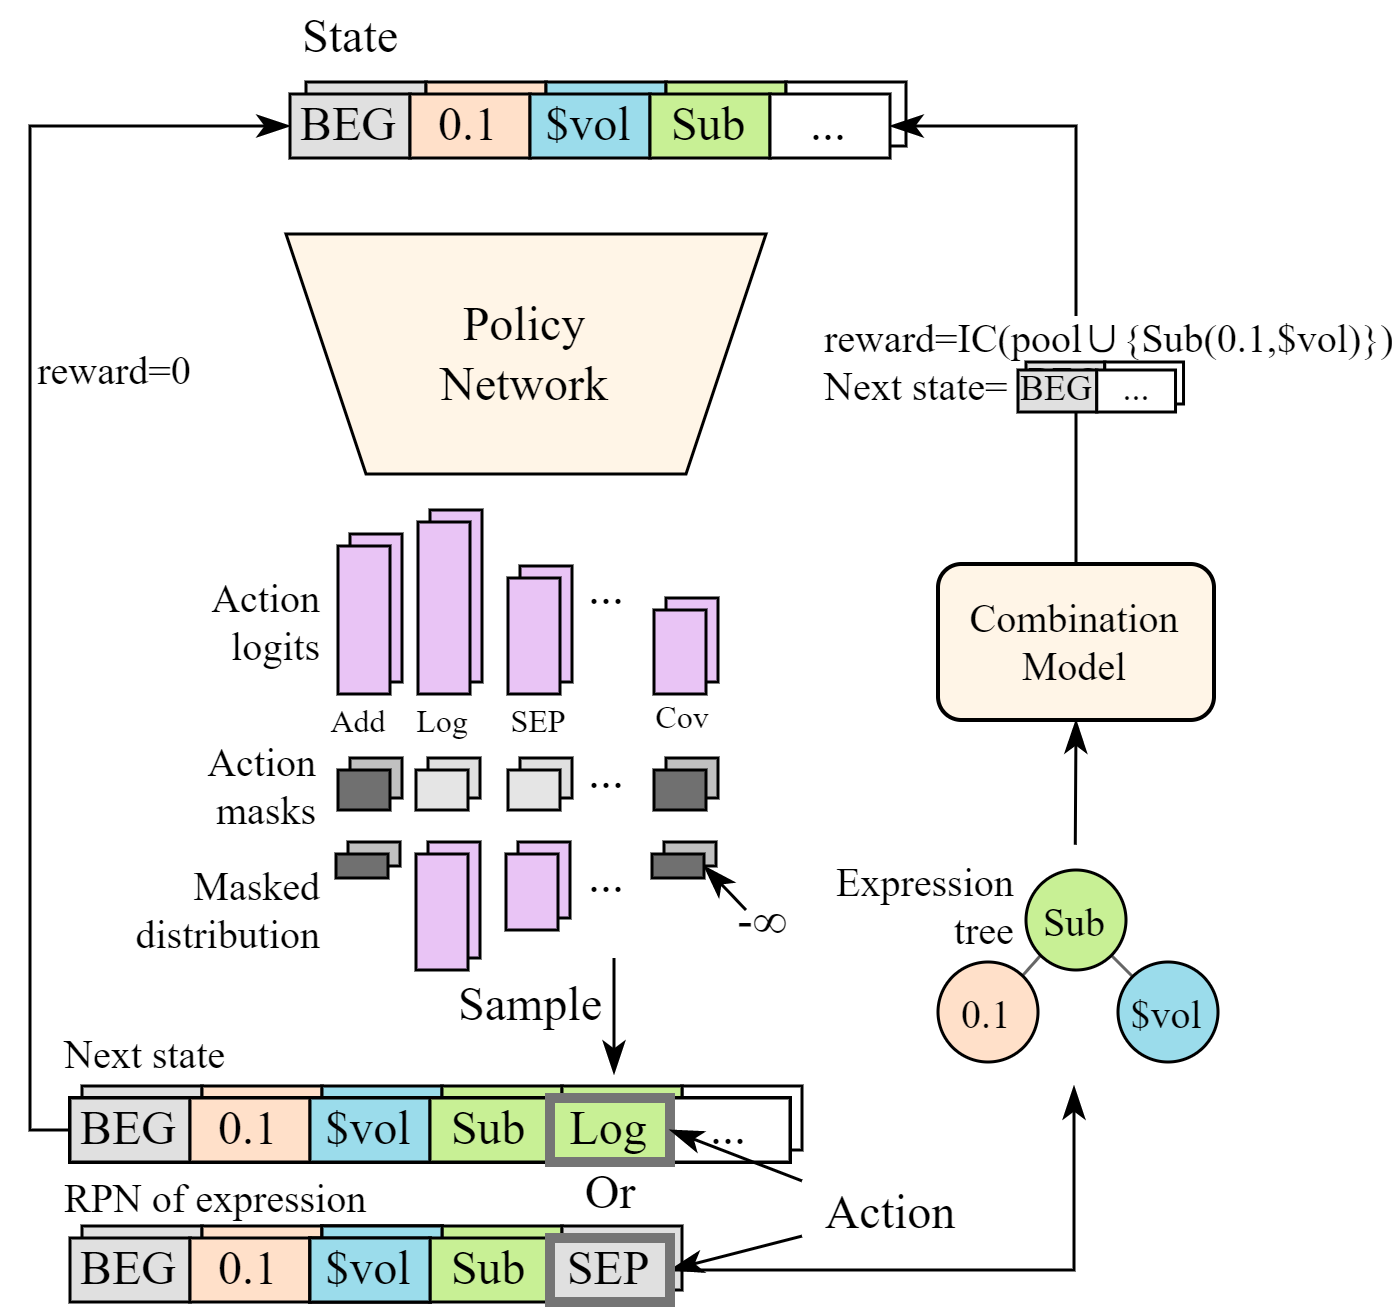
\includegraphics[width=1.0\linewidth]{Images/rl.png}
  \caption{An illustration of our alpha generation framework.}
  \label{fig:rl}
\end{figure}

\subsubsection{State Space}

Each state in the MDP corresponds to a sequence of tokens denoting the currently generated part of the expression. The initial state is always \emph{BEG}, so a valid state always starts with \emph{BEG} and is followed by previously chosen tokens. Since we aim for interpretability of the alphas, and too long of a formula will instead be less interpretable, we cap the length threshold of the formulas at 20 tokens.

\subsubsection{Action Space} \label{sec:action_space}

An action is a token that follows the current state (generated partial sequence). It is obvious that an arbitrarily generated sequence is not guaranteed to be the RPN of an expression, so we only allow a subset of actions to be taken at a specific state to guarantee the well-formedness of the RPN sequence. Please refer to Appendix \ref{sec:expr_legality} for more details.

\subsubsection{Dynamics}

Given a state and an action, we can obtain the next state deterministically. The next state is generated by taking the current state's corresponding sequence and appending the action token at the end.

\subsubsection{Rewards and Returns}

The MDP does not give immediate rewards for partially formed sequences. At the end of each episode, if the final state is valid, the state will be parsed to a formulaic function and evaluated in the combination model shown in Algorithm \ref{alg:model}. To encourage our generator to generate novel alphas, we will then evaluate the new combination model with the new alpha added, and use the model's performance as the return of this episode. Since the reward varies together with the components of the alpha pool, the MDP is non-stationary.

Contrary to common RL task settings, for alpha expression generation we do not necessarily want to penalize longer episodes (longer expressions). In fact, longer alphas that perform well are harder to find than shorter ones, due to exponential explosion of the search space. Consequently, 
we set the discount factor as $\gamma = 1$ (no discount).

\begin{algorithm}
\caption{Alpha Mining Pipeline}
\label{alg:rl}
\KwInput {Stock trend dataset $Y = \braces{y_t}$}
\KwOutput {Optimal alpha subset $F^* = \braces{f_1', \cdots, f_k'}$, optimal weights $w^* = \braces{w_1', \cdots, w_k'}$}
Initialize $\mathcal{F}$ and $w$;\\
Initialize RL policy $\pi_{\theta}$ with parameters $\theta$ and replay buffer $\mathcal{D}$;\\
\For{each iteration}{
    \For{each environment step}{
        $a_t \sim \pi_{\theta}(a_t | s_t)$;\\
        $s_{t+1} \gets [s_t, a_t]$;\\
        \eIf {$a_t = \emph{SEP}\ or\ len(s_{t+1}) \ge threshold$}{
            $f \gets parse(s_{t+1})$;\\
            Update $\mathcal{F}$, $w$ using $f$ and Algorithm \ref{alg:model};\\
            $IC_{new} \gets \bar{\sigma}_y(\sum_{i=1}^{k} w_i f_i)$;\\
            $r_t \gets IC_{new}$;
        }{
            $r_t \gets 0$;
        }
        $\mathcal{D} \gets \mathcal{D} \cup \braces{(s_t, a_t, r_t, s_{t+1})}$;
    }
    \For{each gradient step}{
        Use batch $\mathcal{B} \subset \mathcal{D}$ to do gradient descent on PPO objective $\mathcal{L}^{CLIP}(\theta)$ to update $\theta$;
    }
}
\Return $\mathcal{F}, w$;
\end{algorithm}

\subsubsection{Reinforcement Algorithm}

Based on the MDP defined above, we use Proximal Policy Optimization (PPO) \cite{ppo} to optimize a policy $\pi_\theta(a_t | s_t)$ that takes a state as input and outputs a distribution of action. An actual action will be sampled from the output distribution.

PPO is an on-policy RL algorithm based on the trust region method. It proposed a clipped objective $\mathcal{L}^{CLIP}$ as follows:

\begin{equation}
    \mathcal{L}^{CLIP}(\theta) = \hat{\mathbb{E}}_{t}\brackets{\min\braces{r_t(\theta)\hat{A}_{t},\mathrm{clip}\parens{r_t(\theta), 1-\epsilon, 1+\epsilon}\hat{A}_{t}}},
\end{equation}
where $r_t(\theta)=\frac{\pi_\theta(a_t | s_t)}{\pi_{old}(a_t | s_t)}$ and $\hat{A}_t$ is an estimator of the advantage function at timestep $t$. Using the importance sampling mechanism, PPO can effectively take the biggest possible improvement while keeping the policy in a trust region that avoids accidental performance collapse.

Since our MDP has complicated rules for the legality of actions, an action sampled from the full discrete action distribution predicted by the learned policy is likely to be invalid as mentioned in Section \ref{sec:action_space}. We adopt the Invalid Action Masking mechanism \cite{ppomask} to mask out invalid actions and just sample from the set of valid actions.

\subsection{Network Architecture}

The PPO algorithm requires the agent to have a value network and a policy network. Under our experiment settings, the two networks share a base LSTM feature extractor that converts token sequences into dense vector representations. Separate value and policy ``heads'' are attached after the LSTM. The values of hyperparameters are given in Appendix \ref{sec:hyperparam}.

\subsection{Training with policy gradient-based methods}

For the task of alpha mining, we do not require the agent to achieve relatively high average returns in each episode, but place more importance on the trajectories the agent takes in the whole training process. For this reason, we maintain a pool of alphas without resetting between episodes. We run the alpha generation procedure mentioned in Section \ref{sec:alpha_generation} and optimize the alpha combination model according to Section \ref{sec:alpha_improvement} repeatedly. In this way, we train the policy to continuously generate novel alpha factors that bring improvement to the overall prediction performance.

The proposed alpha mining process is shown in Algorithm \ref{alg:rl}. Our implementation is publicly available\footnote{ \url{https://github.com/RL-MLDM/alphagen/}}.

